\section{Projeto de Controle}

\subsection{Modelagem Térmica do Sistema}

O primeiro passo para a implementação do controle de temperatura da fermentação é a modelagem térmica do processo. Nota-se que essa modelagem é bastante complexa pois envolve diversos coeficientes térmicos desconhecidos, devido a composição heterogênea do Mosto com Leveduras. 

O objetivo do sistema é controlar a temperatura do líquido fermentado (solução de mosto e leveduras). O líquido estará dentro de um fermentador, sem entrada de ar dado que a fermentação é anaeróbica e o ar interfere na qualidade do experimento. Para expulsar o $CO_2$ gerado pela fermentação e não permitir a entrada de $O_2$ o fermentador utiliza um Air-Lock, dispositivo que funciona como válvula só permitindo a direção única desse fluxo. O fermentador será embalado em uma manta térmica, com a intenção de evitar a troca térmica com o ambiente.

Na maior parte das receitas, a fermentação ocorre em temperaturas entre 14°C e 20°C, temperaturas muitas vezes inferiores à temperatura do ambiente. Sendo assim, existe a necessidade de criar um sistema que troque calor com o mosto e leveduras mantendo um gradiente de temperatura entre o fermentador e o ambiente constante conforme configuração do usuário. 

Para isso acontecer durante o processo, o calor retirado pela refrigeração deve ser o mesmo que o gerado pela convecção com o ambiente e pelo próprio processo de fermentação, que é exotérmico. 


É importante destacar que o dispositivo irá ter duas funções: a primeira será manter a temperatura do líquido fermentado; a segunda será levar o líquido até determinada temperatura. Ambas as funcionalidades envolvem a capacidade do dispositivo de retirar ou fornecer calor do sistema de forma eficiente e constante. 


\subsection{Transferência de Calor entre Ar e Fermentador}

Nessa modelagem, serão analisados os seguintes elementos: 
\begin{itemize}
    \item Mosto e Leveduras 
    \item Tanque de Fermentação 
    \item Manta Térmica 
\end{itemize}

Nessa dinâmica, considerando que o fermentador vai operar na maior parte do tempo em temperaturas inferiores às do ambiente, o calor vai fazer o seguinte caminho:
\begin{enumerate}
    \item A manta térmica recebe calor do ambiente através da convecção e radiação do ar. 
    \item A manta térmica transfere calor por condução para o fermentador. 
    \item O fermentador transfere calor por condução para o líquido fermentado. 
    \item O líquido fermentado produz calor pelo processo de fermentação (processo exotérmico).
\end{enumerate}

\begin{center}
    \(Ambiente \longrightarrow Manta\;t\acute{e}rmica \longrightarrow Fermentador \longrightarrow Mosto\;e\;leveduras\)
\end{center}



    
Algumas hipóteses foram adotadas visando simplificar o problema: 

\begin{enumerate}
    \item O gradiente de temperatura no interior do Mosto + Leveduras é desprezível; 
    \item O coeficiente de troca de calor por convecção entre o Mosto + leveduras e o tanque é elevados o bastante para que não sejam observadas diferenças de temperatura entre esses elementos; 
    \item O regime é permanente e as propriedades são constantes 
    \item A condução é unidimensional no plano X
    \item A transferência de calor por radiação é desprezível nas superfícies 
    \item Resistências de contato desprezíveis.
\end{enumerate}


As hipóteses 1, 2, 3  podem ser adotadas devido ao horizonte de tempo da fermentação, no qual é necessário manter a mesma temperatura durante dias. As hipóteses 4, 5 e 6 foram adotadas com a intenção de simplificar o problema. A figura \ref{fig:fermentador_controle} exemplifica esse problema e a figura \ref{fig:fermentador_circuito} demonstra o circuito elétrico equivalente, cuja legenda se encontra na tabela \ref{tab:variaveis_circuito}.

\begin{figure}[h]
    \centering
    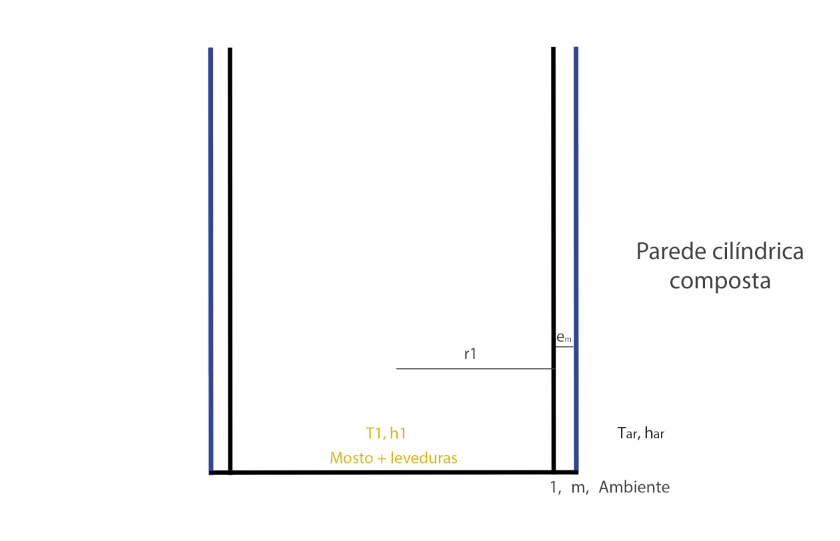
\includegraphics[scale=0.45]{figuras/projeto/controle/fermentador_controle.png}
    \captionsource{Desenho do problema de troca de calor entre o ambiente e fermentador.}{Autores}
    \label{fig:fermentador_controle}
\end{figure}



\subsection{Simulação Térmica}

A Simulação térmica do sistema possui três objetivos:

\begin{enumerate}
    \item Estimar a potência de troca de calor necessária para manter o sistema com 10°C de diferença em relação à temperatura ambiente;
    \item Estimar o tempo morto do sistema para levar o sistema do equilíbrio térmico para uma diferença de 10°C;
    \item Simular um controle PID utilizando uma fonte de calor variável, no caso do sistema real, uma pastilha de Peltier para a sintonização inicial do sistema.
\end{enumerate}

Com esses testes será possível entender se a utilização de pastilhas de Peltier será suficiente para o controle de temperatura.


Foi utilizada a biblioteca Simscape do software Matlab. Essa biblioteca contém blocos que simulam elementos térmicos e funcionam de maneira análoga a um circuito elétrico. No caso, a diferença de temperatura seria equivalente à diferença de potencial elétrico e o calor que circula no sistema seria equivalente a corrente elétrica. As figuras \ref{fig:sim_fonte_calor} a \ref{fig:sim_sensor} representam blocos utilizados.


\begin{figure}[H]
    \centering
    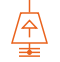
\includegraphics[scale=1.0]{figuras/projeto/controle/fonte_calor.png}
    \caption{Bloco de fonte de calor, que mantém a temperatura em um ponto do circuito constante.}
    \label{fig:sim_fonte_calor}
\end{figure}

\begin{figure}[H]
    \centering
    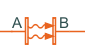
\includegraphics[scale=1.0]{figuras/projeto/controle/conveccao.png}
    \caption{Bloco de transferência de calor por convecção, seguindo a fórmula \(Q = k \cdot A \cdot (T_A - T_B) \)}
    \label{fig:sim_conveccao}
\end{figure}

\begin{figure}[H]
    \centering
    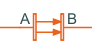
\includegraphics[scale=1.0]{figuras/projeto/controle/radiacao.png}
    \caption{Bloco de transferência de calor por radiação, seguindo a fórmula \(Q = k \cdot A \cdot (T_A^4 - T_B^4) \)}
    \label{fig:sim_radiacao}
\end{figure}

\begin{figure}[H]
    \centering
    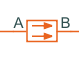
\includegraphics[scale=1.0]{figuras/projeto/controle/conducao.png}
    \caption{Bloco de transferência de calor por condução, seguindo a fórmula \(Q = k \cdot \dfrac{A}{D} (T_A - T_B) \)}
    \label{fig:sim_conducao}
\end{figure}

\begin{figure}[H]
    \centering
    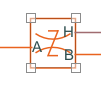
\includegraphics[scale=0.8]{figuras/projeto/controle/sensor_ideal.png}
    \caption{Bloco de sensor de calor ideal}
    \label{fig:sim_sensor}
\end{figure}

\begin{table}[H]
    \begin{center}
        \begin{tabular}{ |c|c| } 
            \hline
            Símbolo & Descrição \\
            \hline
            \(Q\) & Quantidade de Calor \\
            \hline
            \(k\) & Coeficiente de condutividade térmica do material \\
            \hline
            \(A\) & Área normal à transmissão de calor \\
            \hline
            \(D\) & Espessura do material \\
            \hline
            \(T_A, T_B\) & Temperaturas da camada A e B, respectivamente \\
            \hline
        \end{tabular}
        \caption{\label{tab:legenda_blocos} Descrição dos símbolos de trocas de calor referentes às figuras \ref{fig:sim_conveccao} a \ref{fig:sim_conducao}.}
    \end{center}
\end{table}


Com as devidas simplificações justificadas anteriormente, o sistema foi simulado com o circuito da figura \ref{fig:sim_circuito}. A seguir, cada seção de blocos do circuito é descrita em detalhes. A temperatura ambiente adotada na simulação é 25°C e a temperatura do líquido, 15°C.

\begin{figure}[H]
    \centering
    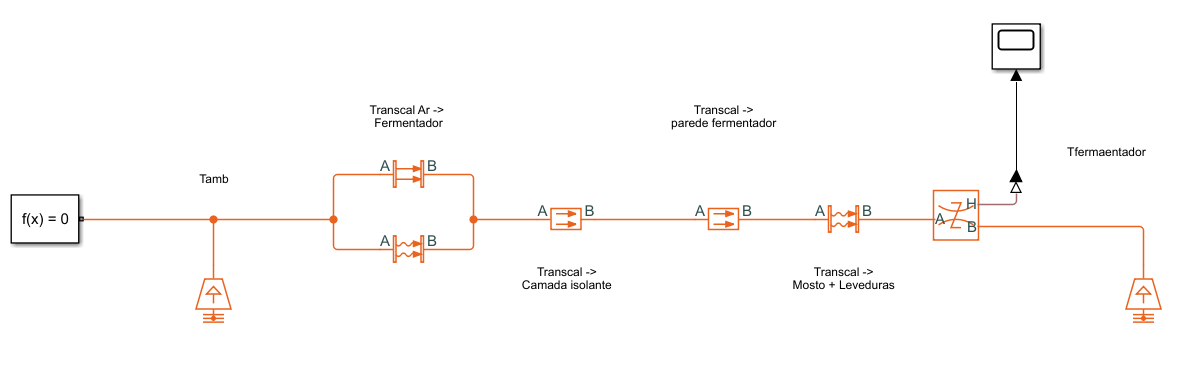
\includegraphics[scale=0.39]{figuras/projeto/controle/sim_circuito.png}
    \captionsource{Circuito de blocos utilizado para a simulação térmica.}{Autores}
    \label{fig:sim_circuito}
\end{figure}


Para a simulação, foi considerado um fermentador cilíndrico com 37 cm de altura e 26 cm de raio. Ele tem paredes de polipropileno com coeficiente térmico de \(0,25 W / m \cdot K\)  e 0,1 cm de espessura. Esse fermentador será encoberto por uma camada de isolante de espuma de poliestireno com coeficiente térmico de  \(0,03 W / m \cdot K\) e 0,2 cm de espessura. O líquido será considerado como água, visando simplificar os cálculos. 


O conjunto de blocos da figura \ref{fig:transcal_amb} representa a transferência de calor entre o ar e a camada isolante que circunda o fermentador. Foram consideradas duas formas de transferência, por convecção e radiação. A área de contato adotada foi \(2 \pi \cdot 0,37 ]cdot 0,263 m^2\), o coeficiente de radiação, \( 5,667 e^{-8} \cdot 0,7 W / m^2 \cdot K^4 \), e o coeficiente de convecção, \(25 W /m^2 \cdot K\) (ar).

\begin{figure}[H]
    \centering
    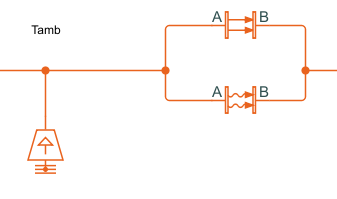
\includegraphics[scale=0.6]{figuras/projeto/controle/transcal_amb.png}
    \caption{Seção do circuito da figura \ref{fig:sim_circuito} referente à transferência de calor entre ambiente e isolamento do fermentador.}
    \label{fig:transcal_amb}
\end{figure}


O bloco da figura \ref{fig:transcal_isolante} representa a transferência de calor por condução entre as paredes do isolante térmico que circunda o fermentador. Foi considerada área de \(2\pi \cdot 0,37 \cdot 0,263 m^2\), espessura de 0,2 cm e coeficiente térmico de condução, \(0.03 W / m \cdot K\).

\begin{figure}[H]
    \centering
    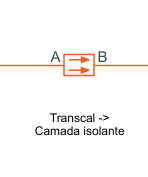
\includegraphics[scale=0.8]{figuras/projeto/controle/transcal_isolante.png}
    \caption{Seção do circuito da figura \ref{fig:sim_circuito} referente à transferência de calor pelo isolamento do fermentador.}
    \label{fig:transcal_isolante}
\end{figure}


A transferência entre extremidades da parede do fermentador é simbolizada pelo bloco da figura \ref{fig:transcal_fermentador}. Para esse bloco, foi adotada área de \(2\pi \cdot 0,37 \cdot 0,261 m^2\), espessura de 0,1 cm e coeficiente térmico de condução, \(0.25 W / m \cdot K\).

\begin{figure}[H]
    \centering
    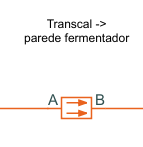
\includegraphics[scale=0.8]{figuras/projeto/controle/transcal_fermentador.png}
    \caption{Seção do circuito da figura \ref{fig:sim_circuito} referente à transferência de calor pelas paredes do fermentador.}
    \label{fig:transcal_fermentador}
\end{figure}


Finalmente, a transferência de calor entre a parede do fermentador e do mosto em fermentação está representado pelo bloco de transferência de calor da figura \ref{fig:transcal_mosto}. Para a simulação foram considerados os valores de área como \(2\pi \cdot 0,37 \cdot 0,261 m^2\) e coeficiente 1000 W / m²·K (considerando a referência da água). 

\begin{figure}[H]
    \centering
    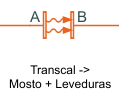
\includegraphics[scale=0.8]{figuras/projeto/controle/transcal_mosto.png}
    \caption{Seção do circuito da figura \ref{fig:sim_circuito} referente à transferência de calor entre paredes do fermentador e mosto em fermentação.}
    \label{fig:transcal_mosto}
\end{figure}


Executando a simulação, a curva de calor resultante (figura \ref{fig:curva_calor}) indica que para manter a temperatura sistema 10°C abaixo do ambiente, é necessário retirar cerca de 57 W de calor do sistema. Esse valor é compatível com a potência máxima das pastilhas de Peltier disponíveis no mercado, que variam entre 90 e 230 W.

\begin{figure}[h]
    \centering
    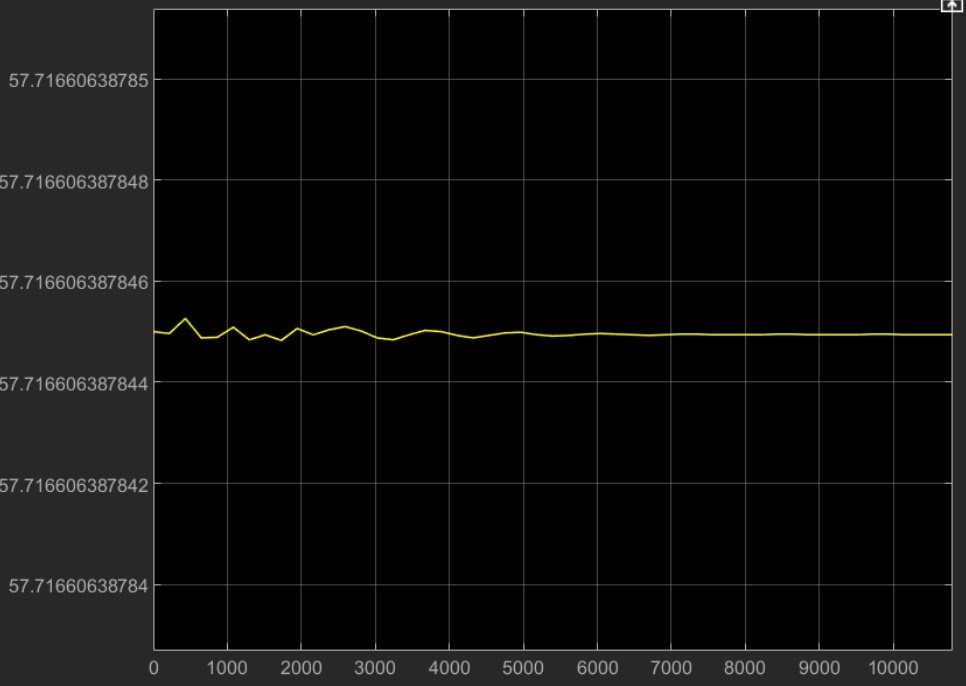
\includegraphics[scale=0.30]{figuras/projeto/controle/curva_calor.jpg}
    \captionsource{Curva de calor obtida a partir da simulação do circuito da figura \ref{fig:sim_circuito}.}{Autores}
    \label{fig:curva_calor}
\end{figure}


Uma segunda simulação foi realizada para determinar o tempo necessário para levar temperatura do sistema do  equilíbrio térmico até uma novo valor. Para isso é ligada uma massa térmica, com o calor específico igual à água de \( 4184 J/K \cdot Kg \), ocupando de 15L do fermentador, e com massa de aproximadamente 15 Kg. O atuador será uma fonte de calor variável, que irá retirar do sistema uma quantidade de calor constante de 57 W. Simulando para intervalo de tempo de 20 horas, foram obtidas as curvas de temperatura (figura \ref{fig:curva_temp}) e quantidade de calor (figura \ref{fig:curva_q}).


\begin{figure}[H]
    \centering
    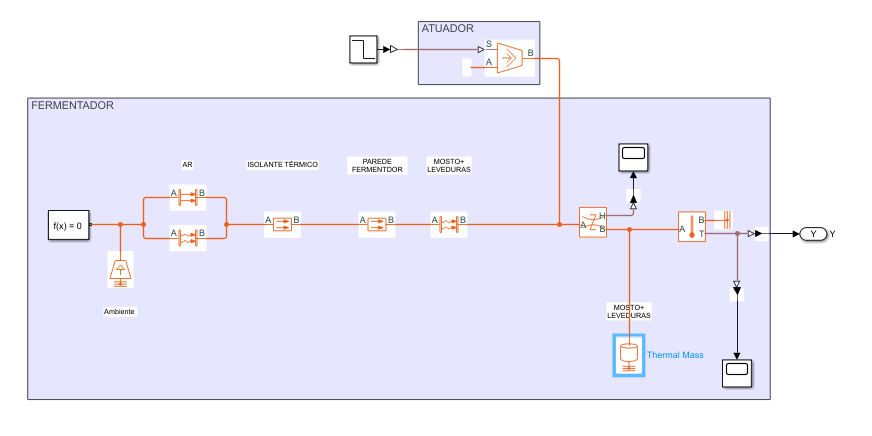
\includegraphics[scale=0.50]{figuras/projeto/controle/circ_atuador.png}
    \captionsource{Circuito térmico completo, com atuador e massa térmica.}{Autores}
    \label{fig:circ_atuador}
\end{figure}


Observando o sistema, conclui-se que o tempo necessário para mover o sistema do equilíbrio térmico para uma temperatura alvo é muito alto e isso pode ser prejudicial nas primeiras horas da fermentação. Dessa forma, é interessante iniciar o processo com a primeira temperatura alvo, o que já é de certa forma realizado na prática, pois a temperatura de início da fermentação deve ser atingida antes do inoculação da levedura e fechamento do fermentador.


\begin{figure}[H]
    \centering
    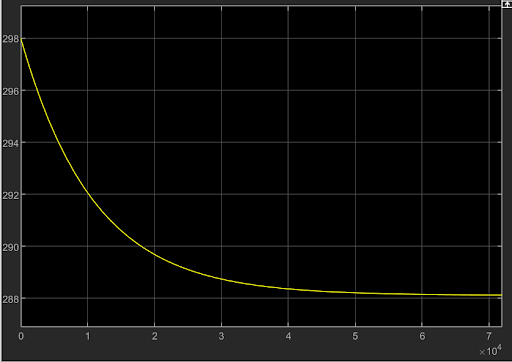
\includegraphics[scale=0.60]{figuras/projeto/controle/curva_temp.png}
    \captionsource{Curva de temperatura em Kelvin por tempo em dezenas de milhares de segundos, obtida da simulação do circuito térmico da figura.}{Autores}
    \label{fig:curva_temp}
\end{figure}

\begin{figure}[H]
    \centering
    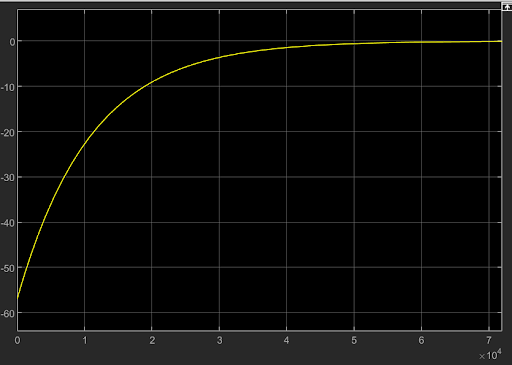
\includegraphics[scale=0.60]{figuras/projeto/controle/curva_q.png}
    \captionsource{Curva de quantidade de calor em Watts por tempo em dezenas de milhares de segundos, obtida da simulação do circuito térmico da figura.}{Autores}
    \label{fig:curva_q}
\end{figure}

\subsection{Dispositivo para Troca de Calor}

Um dos maiores desafios do projeto é criar um sistema que consiga trocar calor de forma eficiente, não seja intrusivo e consiga ser simples o suficiente para ser utilizado por um hobbysta. Conforme anteriormente especificado, a ideia é utilizar placas de peltier para realizar essa troca. A maior vantagem do uso dessas placas é a possibilidade de controlar o calor associado proporcionalmente a quantidade de corrente fornecida ao módulo, através da seguinte equação \ref{eq:qp}. Possibilitando assim o uso de um circuito junto com o microcontrolador para o controle de temperatura.

\begin{equation}
    Q_P = \pi \cdot 1
    \label{eq:qp}
\end{equation}


\subsection{Controle de Temperatura}

Um controlador de malha fechada proporcional interativo derivativo (PID) será utilizado para controlar a temperatura do fermentador. Esse método é amplamente utilizado na indústria, possuindo boa precisão e confiabilidade, além de ser facilmente sintonizado. Inicialmente são definidos parâmetros analógicos e depois é criado o controle digital.

\subsubsection{Controlador PID}

O controlador PID utiliza 3 ações (proporcional, integrativa e derivativa) controlar a planta minimizando o erro. Sua saída pode ser definida pela equação \ref{eq:pid}. A figura \ref{fig:pid} esquematiza a malha de controle.

\begin{equation}
    u(t) = K_pe(t) + K_i  \int_{0}^{t} e(\tau) \, d\tau + K_d\dfrac{de(t)}{\, dt}
    \label{eq:pid}
\end{equation}

Na qual:

\begin{table}[H]
    \begin{center}
        \begin{tabular}{ |c|c| } 
            \hline
            Símbolo   &  Descrição  \\
            \hline
            \(K_p\)   &  ganho proporcional  \\
            \hline
            \(K_i\)   &  ganho integrativo  \\
            \hline
            \(K_d\)   &  ganho derivativo  \\
            \hline
            \(e\)   &  erro  \\
            \hline
            \(t\)   &  tempo  \\
            \hline
            \(\tau\)   &  tempo de integração \\
            \hline
        \end{tabular}
        \caption{\label{tab:variaveis_pid}Descrição das variáveis do controlador PID da Equação \ref{eq:pid}.}
    \end{center}
\end{table}

\begin{figure}[h]
    \centering
    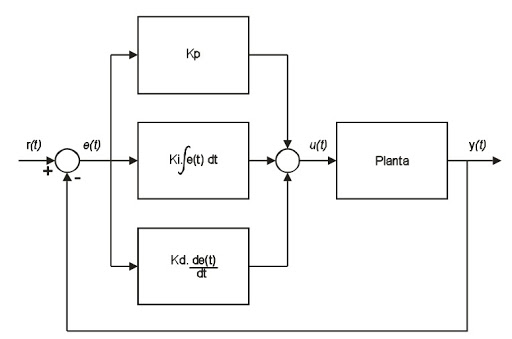
\includegraphics[scale=0.60]{figuras/implementacao/hardware/pid.jpg}
    \caption{Malha de controle PID.}
    \label{fig:pid}
\end{figure}


A ação proporcional do controlador produz um sinal de saída proporcional à amplitude do erro $e(t)$. Essa ação é útil para criar uma resposta equivalente ao tamanho do erro do sistema. A ação integral produz um sinal de saída proporcional à magnitude do erro, dependendo não só do seu valor, mas também da sua duração. Essa ação corrige o erro de off-set gerado pela ação proporcional e acelera a resposta do sistema. Por fim, a ação derivativa produz um sinal de saída proporcional à velocidade de variação do erro. Essa ação melhora a estabilidade e velocidade de resposta do sistema através de uma correção antecipada do erro. 


\subsubsection{Método de Ziegler-Nichols}


Para escolha dos parâmetros de ganho, o método de Ziegler-Nichols foi utilizado. Esse método foi escolhido principalmente pela sua simplicidade e facilidade na sintonização, visto que não é necessário uma modelagem matemática precisa da planta para o seu ajuste. 
A escolha dos parâmetros é feita a partir da observação da resposta do sistema em malha aberta com a aplicação de um degrau. A figura \ref{fig:resposta_sistema} ilustra a curva de resposta do sistema, e a tabela \ref{tab:parametros_ziegler} lista os parâmetros provenientes do método.


\begin{figure}[h]
    \centering
    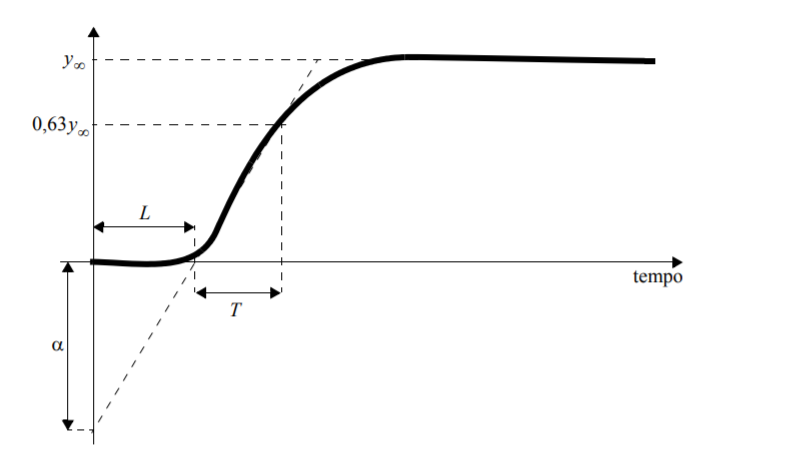
\includegraphics[scale=0.45]{figuras/implementacao/hardware/resposta.png}
    \caption{Responda do Sistema em malha aberta a sinal degrau.}
    \label{fig:resposta_sistema}
\end{figure}

\begin{table}[H]
    \begin{center}
        \begin{tabular}{ |c|c|c|c| } 
            \hline
            Controlador & \(K_p\) & \(T_I\) & \(T_D\) \\
            \hline
            \(P\) & \(1/\alpha\) &  & \\
            \hline
            \(P + I\) & \(0,9/\alpha\) & \(3L\) & \\
            \hline
            \(P + I + D\) & \(1,2/\alpha\) & \(2L\) & \(0,5L\) \\
            \hline
        \end{tabular}
        \caption{\label{tab:parametros_ziegler} Parâmetros do controlador PID seguindo método de Ziegler-Nichols.}
    \end{center}
\end{table}


\subsubsection{Anti Wind-up}

Nesta aplicação, devido a limitações do atuador, é esperado uma saturação na saída. No caso onde o sistema não consegue chegar no setpoint, teremos uma situação chamada de wind-up, na qual, a sua resposta integral irá crescer de forma indefinida. Para evitar problemas no controlador, é necessário a implementação de um sistema anti wind-up, no caso, a ação escolhida será congelar a ação do controlador em caso de saturação.  

